% This file was created with tikzplotlib v0.10.1.
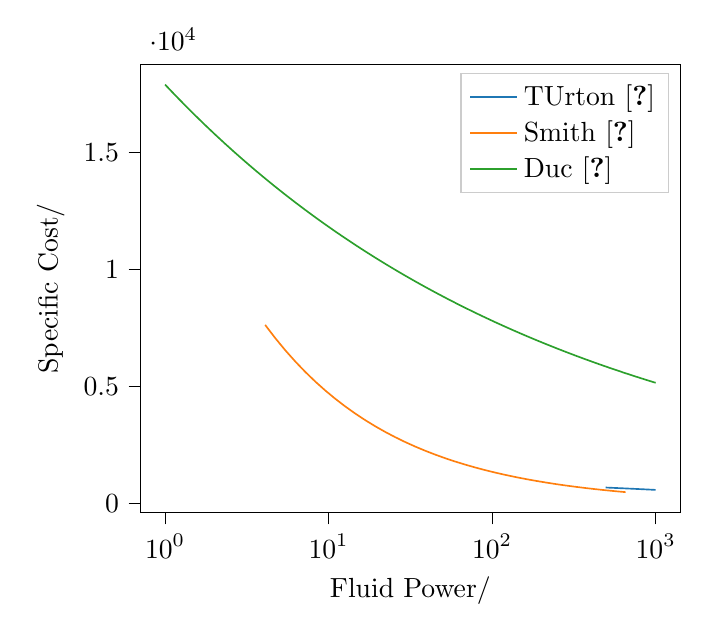
\begin{tikzpicture}

\definecolor{darkgray176}{RGB}{176,176,176}
\definecolor{darkorange25512714}{RGB}{255,127,14}
\definecolor{forestgreen4416044}{RGB}{44,160,44}
\definecolor{lightgray204}{RGB}{204,204,204}
\definecolor{steelblue31119180}{RGB}{31,119,180}

\begin{axis}[
legend cell align={left},
legend style={fill opacity=0.8, draw opacity=1, text opacity=1, draw=lightgray204},
log basis x={10},
tick align=outside,
tick pos=left,
unbounded coords=jump,
x grid style={darkgray176},
xlabel={Fluid Power/\unit{\kilo\watt}},
xmin=0.707945784384138, xmax=1412.53754462275,
xmode=log,
xtick style={color=black},
xtick={0.01,0.1,1,10,100,1000,10000,100000},
xticklabels={
  \(\displaystyle {10^{-2}}\),
  \(\displaystyle {10^{-1}}\),
  \(\displaystyle {10^{0}}\),
  \(\displaystyle {10^{1}}\),
  \(\displaystyle {10^{2}}\),
  \(\displaystyle {10^{3}}\),
  \(\displaystyle {10^{4}}\),
  \(\displaystyle {10^{5}}\)
},
y grid style={darkgray176},
ylabel={Specific Cost/\unit{\USD\per\kilo\watt}},
ymin=-377.460048388404, ymax=18761.4829931995,
ytick style={color=black}
]
\addplot [semithick, steelblue31119180]
table {%
1 nan
1.15139539932645 nan
1.32571136559011 nan
1.52641796717523 nan
1.75751062485479 nan
2.02358964772516 nan
2.32995181051537 nan
2.68269579527973 nan
3.08884359647748 nan
3.55648030622313 nan
4.09491506238043 nan
4.71486636345739 nan
5.42867543932386 nan
6.25055192527397 nan
7.19685673001152 nan
8.28642772854684 nan
9.54095476349994 nan
10.9854114198756 nan
12.648552168553 nan
14.5634847750124 nan
16.7683293681101 nan
19.3069772888325 nan
22.2299648252619 nan
25.5954792269954 nan
29.4705170255181 nan
33.9322177189533 nan
39.0693993705462 nan
44.9843266896945 nan
51.7947467923121 nan
59.6362331659464 nan
68.66488450043 nan
79.060432109077 nan
91.0298177991522 nan
104.811313415469 nan
120.679264063933 nan
138.949549437314 nan
159.985871960606 nan
184.206996932672 nan
212.095088792019 nan
244.205309454865 nan
281.176869797423 nan
323.745754281764 nan
372.759372031494 nan
429.193426012878 nan
494.171336132383 689.532496796874
568.986602901829 670.437342031996
655.128556859551 650.716356463205
754.312006335462 630.456783338788
868.511373751352 609.746043754091
1000 588.671121693816
};
\addlegendentry{TUrton \cite{Turton2012}}
\addplot [semithick, darkorange25512714]
table {%
1 nan
1.15139539932645 nan
1.32571136559011 nan
1.52641796717523 nan
1.75751062485479 nan
2.02358964772516 nan
2.32995181051537 nan
2.68269579527973 nan
3.08884359647748 nan
3.55648030622313 nan
4.09491506238043 7631.38177943684
4.71486636345739 7071.99518482377
5.42867543932386 6553.61209013728
6.25055192527397 6073.22690492807
7.19685673001152 5628.05435101204
8.28642772854684 5215.51331339903
9.54095476349994 4833.21187496192
10.9854114198756 4478.93344807684
12.648552168553 4150.62392282555
14.5634847750124 3846.37975724532
16.7683293681101 3564.43694057328
19.3069772888325 3303.16076549408
22.2299648252619 3061.0363500903
25.5954792269954 2836.65985454165
29.4705170255181 2628.7303416475
33.9322177189533 2436.04223397969
39.0693993705462 2257.47832393245
44.9843266896945 2092.00329614127
51.7947467923121 1938.65772471395
59.6362331659464 1796.5525104695
68.66488450043 1664.86372593208
79.060432109077 1542.82783819109
91.0298177991522 1429.73728192965
104.811313415469 1324.93635695365
120.679264063933 1227.8174264354
138.949549437314 1137.81739382912
159.985871960606 1054.41443803144
184.206996932672 977.124987857349
212.095088792019 905.500918289545
244.205309454865 839.12695224504
281.176869797423 777.61825279441
323.745754281764 720.618191873368
372.759372031494 667.796282549626
429.193426012878 618.846262856302
494.171336132383 573.484320081929
568.986602901829 531.447445221464
655.128556859551 492.49190804741
754.312006335462 nan
868.511373751352 nan
1000 nan
};
\addlegendentry{Smith \cite{Smith2005}}
\addplot [semithick, forestgreen4416044]
table {%
1 17891.5310367637
1.15139539932645 17443.2376600146
1.32571136559011 17006.176801669
1.52641796717523 16580.0670177525
1.75751062485479 16164.6339162006
2.02358964772516 15759.6099801654
2.32995181051537 15364.7343957484
2.68269579527973 14979.7528840505
3.08884359647748 14604.4175374299
3.55648030622313 14238.4866598624
4.09491506238043 13881.7246113027
4.71486636345739 13533.9016559438
5.42867543932386 13194.7938142803
6.25055192527397 12864.1827188767
7.19685673001152 12541.855473751
8.28642772854684 12227.6045172803
9.54095476349994 11921.2274885431
10.9854114198756 11622.5270970086
12.648552168553 11331.3109954928
14.5634847750124 11047.3916562968
16.7683293681101 10770.5862504489
19.3069772888325 10500.7165299728
22.2299648252619 10237.608713105
25.5954792269954 9981.09337238855
29.4705170255181 9731.00532557122
33.9322177189533 9487.18352923642
39.0693993705462 9249.47097510003
44.9843266896945 9017.71458890536
51.7947467923121 8791.76513185146
59.6362331659464 8571.47710449126
68.66488450043 8356.70865303766
79.060432109077 8147.32147801722
91.0298177991522 7943.18074521265
104.811313415469 7744.15499883675
120.679264063933 7550.11607688182
138.949549437314 7360.9390285902
159.985871960606 7176.50203399258
184.206996932672 6996.68632546241
212.095088792019 6821.37611123589
244.205309454865 6650.45850084817
281.176869797423 6483.82343243794
323.745754281764 6321.36360187343
372.759372031494 6162.97439365421
429.193426012878 6008.55381354442
494.171336132383 5858.00242289387
568.986602901829 5711.22327460481
655.128556859551 5568.12185070322
754.312006335462 5428.60600147416
868.511373751352 5292.58588612235
1000 5159.97391491938
};
\addlegendentry{Duc \cite{Duc2007}}
\end{axis}

\end{tikzpicture}
